\documentclass[11pt]{article}
\usepackage[a4paper,margin=2.2cm]{geometry}
\usepackage{amsmath,amssymb,amsfonts,mathtools}
\usepackage{bm}
\usepackage{xcolor}
\usepackage{longtable,array}
\usepackage[most]{tcolorbox}
\usepackage{tikz}
\usetikzlibrary{arrows.meta,decorations.pathmorphing}
\usepackage{hyperref}
\hypersetup{colorlinks=true,linkcolor=blue!55!black,urlcolor=blue!55!black}
\allowdisplaybreaks[4]

\tikzset{
  gl/.style={decorate,decoration={coil,aspect=0.55,segment length=2.1mm,amplitude=0.75mm},thick},
  qk/.style={thick,-{Stealth[length=2mm]}},
  val/.style={line width=1.6pt,double,double distance=1.6pt},
  ins/.style={thick},
  cut/.style={dashed,gray!70,line width=0.5pt}
}
\newcommand{\ibar}[2]{\draw[line width=1.1pt] (#1-0.13,#2) -- (#1+0.13,#2);}
\newcommand{\ibarh}[2]{\draw[line width=1.1pt] (#1,#2-0.13) -- (#1,#2+0.13);}
\newcommand{\dg}{\dagger}
\newcommand{\eps}{\varepsilon}
\newcommand{\ip}[1]{\int\!\frac{d^{3}#1}{(2\pi)^{3}}}
\newcommand{\dthree}{\delta^{(3)}}
\newcommand{\ket}[1]{\left|#1\right\rangle}
\newcommand{\bra}[1]{\left\langle#1\right|}
\newcommand{\vac}{\ket{0}}
\newcommand{\A}{\mathcal{A}}\newcommand{\B}{\mathcal{B}}
\newcommand{\C}{\mathcal{C}}\newcommand{\D}{\mathcal{D}}
\newcommand{\qk}[3]{q^{#1}_{#2}(#3)}
\newcommand{\aqk}[3]{\bar q^{#1}_{#2}(#3)}
\newcommand{\gl}[3]{g^{#1}_{#2}(#3)}
\newcommand{\Jc}{\mathcal{J}}

\newtcolorbox{res}[1][]{colback=blue!3,colframe=blue!45!black,boxrule=0.6pt,
  arc=2pt,left=6pt,right=6pt,top=4pt,bottom=4pt,#1}
\newtcolorbox{warn}[1][]{colback=orange!5,colframe=orange!60!black,boxrule=0.6pt,
  arc=2pt,left=6pt,right=6pt,top=4pt,bottom=4pt,#1}
\newtcolorbox{newfind}[1][]{colback=green!4,colframe=green!45!black,boxrule=0.6pt,
  arc=2pt,left=6pt,right=6pt,top=4pt,bottom=4pt,#1}

\title{\bf Instantaneous contributions to the soft quark light-cone wave function:\\
complete enumeration, diagrams and wave functions}
\date{}\author{}

\begin{document}
\maketitle
\vspace{-1.2cm}

\begin{abstract}\noindent
We enumerate every instantaneous contribution to the soft $q\bar q$ sector at $O(g^{2})$ and give
the corresponding diagram and light-cone wave function for each. There are two sources: the
instantaneous gluon exchange, which is a single current--current operator whose cross terms
generate five distinct topologies, and the instantaneous quark exchange, which generates three.
A uniform vertex rule reduces all instantaneous-gluon graphs to one expression. Two of the
topologies --- the $\Jc_{q}\!\cdot\!\Jc_{g}$ cross terms, feeding $\B_{3}$ and $\B_{1}$ --- do not
appear anywhere in the current draft and were also absent from the corrected manuscript.
\end{abstract}

%=====================================================================
\section{Where the instantaneous terms come from}
%=====================================================================

Eliminating the constrained components $A^{-}$ and $\psi_{-}$ in $A^{+}=0$ gauge leaves two
instantaneous operators.

\paragraph{(A) Instantaneous gluon exchange.} This is a single current--current operator,
\begin{equation}
H^{(A)}_{\rm inst}=\frac{g^{2}}{2}\int\! dx^{-}d^{2}x\;
\Jc^{a}\,\frac{1}{(\partial^{+})^{2}}\,\Jc^{a},
\qquad
\Jc^{a}=\underbrace{\rho^{a}}_{\rm valence}
+\underbrace{f^{abc}A^{b}_{i}\partial^{+}A^{c}_{i}}_{\Jc^{a}_{g}}
+\underbrace{\xi^{\dg}t^{a}\xi}_{\Jc^{a}_{q}} .
\label{eq:HinstA}
\end{equation}
Writing $\Jc$ as a sum makes the classification automatic: the cross terms are
\begin{center}
\renewcommand{\arraystretch}{1.25}
\begin{tabular}{lll}
\hline
cross term & content & status\\
\hline
$\rho\!\cdot\!\rho$ & valence only & no soft dynamics\\
$\rho\!\cdot\!\Jc_{g}$ & $H_{gg\text{-inst}}$ of the pure Yang--Mills paper & already known\\
$\rho\!\cdot\!\Jc_{q}$ & Group \textbf{A} below & partly in the draft\\
$\Jc_{q}\!\cdot\!\Jc_{q}$ & Group \textbf{B} below & missing from the draft\\
$\Jc_{q}\!\cdot\!\Jc_{g}$ & Group \textbf{C} below & \textbf{newly identified}\\
$\Jc_{g}\!\cdot\!\Jc_{g}$ & part of $H_{gggg}+H_{gggg\text{-inst}}$ & pure glue\\
\hline
\end{tabular}
\end{center}

\paragraph{(B) Instantaneous quark exchange.}
\begin{equation}
H_{ggq\bar q}=g^{2}\!\int\! dx^{-}d^{2}x\;
\xi^{\dg}\big(\sigma^{i}A^{i}_{a}t^{a}\big)\frac{1}{2i\partial^{+}}
\big(\sigma^{j}A^{j}_{b}t^{b}\big)\xi ,
\label{eq:Hggqq}
\end{equation}
giving Group \textbf{D}.

%=====================================================================
\section{Conventions}
%=====================================================================

$\eps_{p}=\bm p^{2}/2p^{+}$. The outgoing quark is $(\beta,\lambda_{1},l)$ and the outgoing
antiquark $(\alpha,\lambda_{2},m)$, as in the ansatz. All the wave functions below are
\emph{first order} in perturbation theory --- a single insertion of an instantaneous vertex ---
so in every case
\begin{equation}
\psi=\frac{\bra{f}H_{\rm inst}\ket{i}}{E_{i}-E_{f}} .
\label{eq:PT1}
\end{equation}

\paragraph{Diagram conventions.}
\begin{center}
\begin{tabular}{ll@{\hspace{1.2cm}}ll}
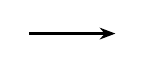
\begin{tikzpicture}[baseline=-2pt]\draw[qk](0,0)--(1.1,0);\end{tikzpicture}
& quark (arrow $=$ fermion flow) &
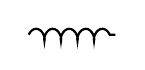
\begin{tikzpicture}[baseline=-2pt]\draw[gl](0,0)--(1.1,0);\end{tikzpicture}
& gluon\\[4pt]
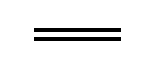
\begin{tikzpicture}[baseline=-2pt]\draw[val](0,0)--(1.1,0);\end{tikzpicture}
& valence source $\rho$ &
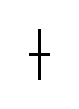
\begin{tikzpicture}[baseline=-2pt]\draw[ins](0.55,-0.3)--(0.55,0.35);\ibar{0.55}{0.02}\end{tikzpicture}
& instantaneous exchange\\[6pt]
\begin{tikzpicture}[baseline=-2pt]\draw[cut](0.55,-0.3)--(0.55,0.35);\end{tikzpicture}
& intermediate state & &\\
\end{tabular}
\end{center}
The bar across a line is the standard light-cone marking for an instantaneous (non-propagating)
exchange: it carries no energy denominator of its own, only the $1/(P^{+})^{2}$ of
Eq.~\eqref{eq:HinstA} or the $1/2P^{+}$ of Eq.~\eqref{eq:Hggqq}.

\subsection{A uniform rule for the instantaneous gluon exchange}

Every graph generated by \eqref{eq:HinstA} has the same form: two ``charges'' joined by a line
carrying longitudinal momentum $P^{+}$,
\begin{equation}
\boxed{\;
\bra{f}H^{(A)}_{\rm inst}\ket{i}=\frac{g^{2}}{(2\pi)^{3}}\;
\frac{\mathcal{Q}^{a}_{(1)}\,\mathcal{Q}^{a}_{(2)}}{(P^{+})^{2}}\;\times
\begin{cases}
1 & \text{if one charge is }\rho,\\[2pt]
\dthree(\Sigma_{\rm in}-\Sigma_{\rm out}) & \text{otherwise,}
\end{cases}}
\label{eq:rule}
\end{equation}
with the charges
\begin{center}
\renewcommand{\arraystretch}{1.5}
\begin{tabular}{ll}
\hline
transition & $\mathcal{Q}^{a}$\\
\hline
valence & $\rho^{a}(\mp k)$\\
$q^{\beta}_{\lambda}(l)\to q^{\beta'}_{\lambda'}(l')$ &
$t^{a}_{\beta'\beta}\,\delta_{\lambda\lambda'}$\\
$\bar q^{\alpha}_{\lambda}(m)\to\bar q^{\alpha'}_{\lambda'}(m')$ &
$-\,t^{a}_{\alpha\alpha'}\,\delta_{\lambda\lambda'}$\\
$0\to q^{\beta}_{\lambda_{1}}(l)\,\bar q^{\alpha}_{\lambda_{2}}(m)$ &
$t^{a}_{\beta\alpha}\,\delta_{\lambda_{1}\lambda_{2}}$\\
$g^{b}_{i}(p)\to g^{c}_{j}(q)$ &
$\dfrac{i f^{abc}(p^{+}+q^{+})\,\delta_{ij}}{2\sqrt{p^{+}q^{+}}}$\\
$0\to g^{b}_{i}(p)\,g^{c}_{j}(q)$ &
$\dfrac{i f^{abc}(q^{+}-p^{+})\,\delta_{ij}}{2\sqrt{p^{+}q^{+}}}$\\
\hline
\end{tabular}
\end{center}
The two last entries are read off from Eqs.~(D.4) and (D.5) of the pure Yang--Mills paper; the
quark entries are fixed by Eq.~(22) of the notes. Note that $8\pi^{3}=(2\pi)^{3}$, so the two
calibrations already agree.

\begin{warn}
\textbf{One caveat on normalization.} Rule \eqref{eq:rule} is calibrated on the two cases in which
one charge is the valence $\rho$ --- Eq.~(22) of the notes and Eqs.~(D.4)/(D.5) of the pure gauge
paper --- and those two agree with each other. For Groups \textbf{B} and \textbf{C}, where
\emph{both} charges are soft, the relative factor between the ``$\rho$ present'' and ``$\rho$
absent'' cases in \eqref{eq:rule} follows from writing \eqref{eq:HinstA} in momentum space as
$\tfrac{g^{2}}{2}\!\int\!\tfrac{d^{3}P}{(2\pi)^{3}}(P^{+})^{-2}\Jc^{a}(-P)\Jc^{a}(P)$, but I have
not been able to check it against an independently normalized expression in either draft. The
colour factors, $P^{+}$ assignments, relative signs and energy denominators below are
unaffected; \emph{confirm the overall constant of Groups B and C against your own derivation of
$H^{(A)}_{\rm inst}$ before using them.}
\end{warn}

%=====================================================================
\section{Group A: valence $\leftrightarrow$ soft quark ($\rho\cdot\Jc_{q}$)}
%=====================================================================

\subsection*{A1. \ $\vac\to\ket{q\bar q}$}
\begin{center}
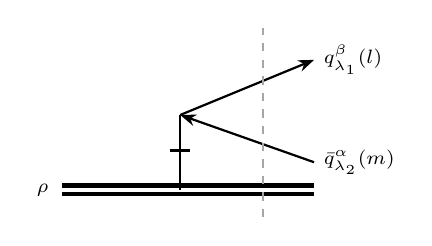
\begin{tikzpicture}
\draw[val] (0,0) -- (3.2,0); \node[left] at (-0.05,0) {\scriptsize$\rho$};
\draw[ins] (1.5,0) -- (1.5,0.95); \ibar{1.5}{0.5}
\draw[qk] (1.5,0.95) -- (3.2,1.65); \node[right] at (3.2,1.65) {\scriptsize$\qk{\beta}{\lambda_{1}}{l}$};
\draw[qk] (3.2,0.35) -- (1.5,0.95); \node[right] at (3.2,0.35) {\scriptsize$\aqk{\alpha}{\lambda_{2}}{m}$};
\draw[cut] (2.55,-0.35) -- (2.55,2.05);
\end{tikzpicture}
\end{center}
$P^{+}=k^{+}=l^{+}+m^{+}$, $E_{i}=0$, $E_{f}=\eps_{l}+\eps_{m}$:
\begin{res}
\begin{equation}
\psi_{\rm A1}=-\,\frac{g^{2}\,t^{a}_{\beta\alpha}\,\rho^{a}(-k)\,\delta_{\lambda_{1}\lambda_{2}}}
{(2\pi)^{3}\,(k^{+})^{2}\,\big(\eps_{l}+\eps_{m}\big)},\qquad k=l+m .
\label{eq:A1}
\end{equation}
\end{res}
\noindent
This is Eq.~(22) of the notes. It feeds $\A_{1}$, and in the combination with the
non-instantaneous graph it cancels the $\delta_{\lambda_{1}\lambda_{2}}/(k^{+})^{2}\eps_{q\bar q}$
piece exactly, leaving the compact two-term $\A_{1}$.

\subsection*{A2. \ $\ket{q\bar q}\to\ket{q\bar q}$, quark leg scatters off the valence}
\begin{center}
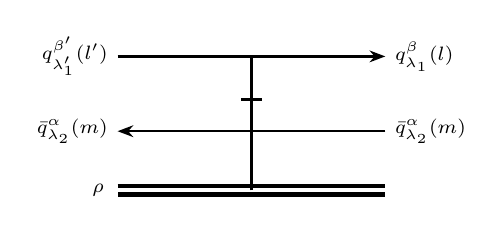
\begin{tikzpicture}
\draw[val] (0,0) -- (3.4,0); \node[left] at (-0.05,0) {\scriptsize$\rho$};
\draw[qk] (0,1.7) -- (3.4,1.7);
\node[left] at (0,1.7) {\scriptsize$\qk{\beta'}{\lambda_{1}'}{l'}$};
\node[right] at (3.4,1.7) {\scriptsize$\qk{\beta}{\lambda_{1}}{l}$};
\draw[qk] (3.4,0.75) -- (0,0.75);
\node[left] at (0,0.75) {\scriptsize$\aqk{\alpha}{\lambda_{2}}{m}$};
\node[right] at (3.4,0.75) {\scriptsize$\aqk{\alpha}{\lambda_{2}}{m}$};
\draw[ins] (1.7,0) -- (1.7,1.7); \ibar{1.7}{1.15}
\end{tikzpicture}
\end{center}
$P^{+}=l'^{+}-l^{+}$, $E_{i}-E_{f}=\eps_{l'}-\eps_{l}$ (the antiquark is a spectator):
\begin{res}
\begin{equation}
\psi_{\rm A2}=\frac{g^{2}\,t^{a}_{\beta\beta'}\,\rho^{a}(l'-l)\,\delta_{\lambda_{1}\lambda_{1}'}\,
\delta^{\alpha\alpha'}\delta_{\lambda_{2}\lambda_{2}'}\dthree(m-m')}
{(2\pi)^{3}\,(l'^{+}-l^{+})^{2}\,\big(\eps_{l'}-\eps_{l}\big)} .
\label{eq:A2}
\end{equation}
\end{res}

\subsection*{A3. \ $\ket{q\bar q}\to\ket{q\bar q}$, antiquark leg scatters off the valence}
\begin{center}
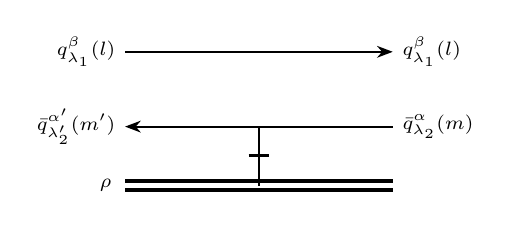
\begin{tikzpicture}
\draw[val] (0,0) -- (3.4,0); \node[left] at (-0.05,0) {\scriptsize$\rho$};
\draw[qk] (0,1.7) -- (3.4,1.7);
\node[left] at (0,1.7) {\scriptsize$\qk{\beta}{\lambda_{1}}{l}$};
\node[right] at (3.4,1.7) {\scriptsize$\qk{\beta}{\lambda_{1}}{l}$};
\draw[qk] (3.4,0.75) -- (0,0.75);
\node[left] at (0,0.75) {\scriptsize$\aqk{\alpha'}{\lambda_{2}'}{m'}$};
\node[right] at (3.4,0.75) {\scriptsize$\aqk{\alpha}{\lambda_{2}}{m}$};
\draw[ins] (1.7,0) -- (1.7,0.75); \ibar{1.7}{0.38}
\end{tikzpicture}
\end{center}
The antiquark charge carries the extra minus sign of the rule:
\begin{res}
\begin{equation}
\psi_{\rm A3}=-\,\frac{g^{2}\,t^{a}_{\alpha'\alpha}\,\rho^{a}(m'-m)\,\delta_{\lambda_{2}\lambda_{2}'}\,
\delta^{\beta\beta'}\delta_{\lambda_{1}\lambda_{1}'}\dthree(l-l')}
{(2\pi)^{3}\,(m'^{+}-m^{+})^{2}\,\big(\eps_{m'}-\eps_{m}\big)} .
\label{eq:A3}
\end{equation}
\end{res}
\noindent
A2 and A3 are the eikonal colour rotation of a soft quark in the valence background. They
populate the $b^{\dg}b$ and $d^{\dg}d$ structures, which are \emph{absent from the ansatz}; within
the $q\bar q$ sector they contribute to $\D_{3}$ through the spectator delta.

\subsection*{A4. \ $\ket{g}\to\ket{g\,q\bar q}$ (spectator gluon)}
\begin{center}
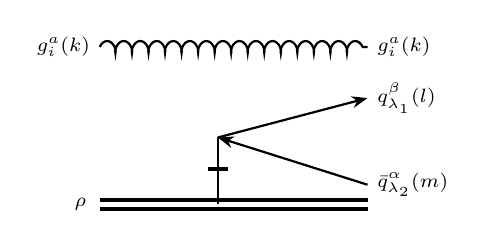
\begin{tikzpicture}
\draw[val] (0,0) -- (3.4,0); \node[left] at (-0.05,0) {\scriptsize$\rho$};
\draw[gl] (0,2.0) -- (3.4,2.0);
\node[left] at (0,2.0) {\scriptsize$\gl{a}{i}{k}$};
\node[right] at (3.4,2.0) {\scriptsize$\gl{a}{i}{k}$};
\draw[ins] (1.5,0) -- (1.5,0.85); \ibar{1.5}{0.45}
\draw[qk] (1.5,0.85) -- (3.4,1.35); \node[right] at (3.4,1.35) {\scriptsize$\qk{\beta}{\lambda_{1}}{l}$};
\draw[qk] (3.4,0.25) -- (1.5,0.85); \node[right] at (3.4,0.25) {\scriptsize$\aqk{\alpha}{\lambda_{2}}{m}$};
\end{tikzpicture}
\end{center}
Identical to A1 times the spectator delta. It is \emph{disconnected} and is already accounted for
by the $\A_{1}$ term in the action of $\Omega$ on $\ket{g}$; it must be subtracted, not added,
when reading off $\B_{3}$.

%=====================================================================
\section{Group B: soft quark $\leftrightarrow$ soft quark ($\Jc_{q}\cdot\Jc_{q}$)}
%=====================================================================

\subsection*{B1. \ $\ket{q\bar q}\to\ket{q\bar q}$, instantaneous gluon between the two legs}
\begin{center}
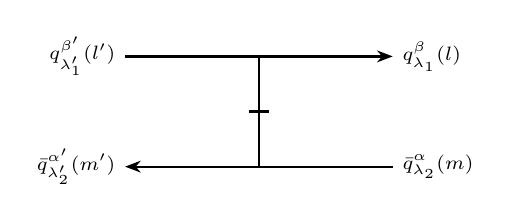
\begin{tikzpicture}
\draw[qk] (0,1.6) -- (3.4,1.6);
\node[left] at (0,1.6) {\scriptsize$\qk{\beta'}{\lambda_{1}'}{l'}$};
\node[right] at (3.4,1.6) {\scriptsize$\qk{\beta}{\lambda_{1}}{l}$};
\draw[qk] (3.4,0.2) -- (0,0.2);
\node[left] at (0,0.2) {\scriptsize$\aqk{\alpha'}{\lambda_{2}'}{m'}$};
\node[right] at (3.4,0.2) {\scriptsize$\aqk{\alpha}{\lambda_{2}}{m}$};
\draw[ins] (1.7,1.6) -- (1.7,0.2); \ibar{1.7}{0.9}
\end{tikzpicture}
\end{center}
$P^{+}=l'^{+}-l^{+}=m^{+}-m'^{+}$; the product of a quark charge and an antiquark charge carries
one minus sign:
\begin{res}
\begin{equation}
\psi_{\rm B1}=-\,\frac{g^{2}\,t^{a}_{\beta\beta'}t^{a}_{\alpha'\alpha}\,
\delta_{\lambda_{1}\lambda_{1}'}\delta_{\lambda_{2}\lambda_{2}'}\,\dthree(l+m-l'-m')}
{(2\pi)^{3}\,(l'^{+}-l^{+})^{2}\,
\big(\eps_{l'}+\eps_{m'}-\eps_{l}-\eps_{m}\big)} .
\label{eq:B1}
\end{equation}
\end{res}
\noindent
This is the instantaneous $\Jc_{q}\!\cdot\!\Jc_{q}$ exchange flagged as missing from the $\D_{3}$
sector. Together with the $t$-channel one-gluon exchange it must satisfy
$X(m',l',m,l)+X^{\dg}(m,l,m',l')=0$, since the $s$-channel graph already saturates the unitarity
relation for $\D_{3}$.

\subsection*{B2. \ $\vac\to\ket{q\bar q\,q\bar q}$}
\begin{center}
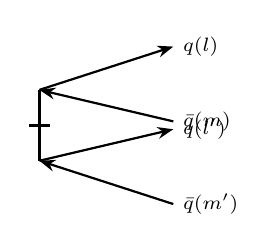
\begin{tikzpicture}
\draw[ins] (1.7,1.35) -- (1.7,0.45); \ibar{1.7}{0.9}
\draw[qk] (1.7,1.35) -- (3.4,1.9); \node[right] at (3.4,1.9) {\scriptsize$q(l)$};
\draw[qk] (3.4,0.95) -- (1.7,1.35); \node[right] at (3.4,0.95) {\scriptsize$\bar q(m)$};
\draw[qk] (1.7,0.45) -- (3.4,0.85); \node[right] at (3.4,0.85) {\scriptsize$q(l')$};
\draw[qk] (3.4,-0.1) -- (1.7,0.45); \node[right] at (3.4,-0.1) {\scriptsize$\bar q(m')$};
\end{tikzpicture}
\end{center}
Both currents create a pair. This is a legitimate $O(g^{2})$ transition, but the structure
$b^{\dg}d^{\dg}b^{\dg}d^{\dg}$ with no gluon operator is \emph{not in the ansatz}; it first
matters when $\Omega$ acts on states containing two pairs. Recorded here for completeness.

%=====================================================================
\section{Group C: soft quark $\leftrightarrow$ soft gluon ($\Jc_{q}\cdot\Jc_{g}$)}
%=====================================================================

\begin{newfind}
\textbf{These two topologies appear nowhere in the draft, and I did not include them in the
corrected manuscript either.} They arise because $\Jc_{g}$ --- the soft gluon colour charge
density in Eq.~\eqref{eq:HinstA} --- can be contracted against the soft quark current, not only
against $\rho$. They are the same order as every other instantaneous term and feed $\B_{3}$ and
$\B_{1}$.
\end{newfind}

\subsection*{C1. \ $\ket{g}\to\ket{q\bar q\,g}$ \quad (feeds $\B_{3}$)}
\begin{center}
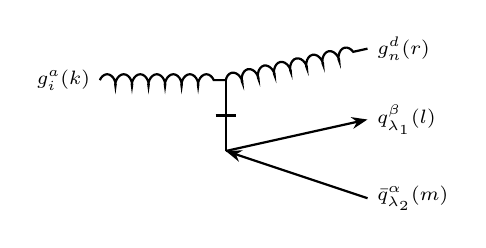
\begin{tikzpicture}
\draw[gl] (0,1.6) -- (1.6,1.6); \node[left] at (0,1.6) {\scriptsize$\gl{a}{i}{k}$};
\draw[gl] (1.6,1.6) -- (3.4,2.0); \node[right] at (3.4,2.0) {\scriptsize$\gl{d}{n}{r}$};
\draw[ins] (1.6,1.6) -- (1.6,0.7); \ibar{1.6}{1.15}
\draw[qk] (1.6,0.7) -- (3.4,1.1); \node[right] at (3.4,1.1) {\scriptsize$\qk{\beta}{\lambda_{1}}{l}$};
\draw[qk] (3.4,0.1) -- (1.6,0.7); \node[right] at (3.4,0.1) {\scriptsize$\aqk{\alpha}{\lambda_{2}}{m}$};
\end{tikzpicture}
\end{center}
Charges: pair creation $t^{b}_{\beta\alpha}\delta_{\lambda_{1}\lambda_{2}}$ and gluon transition
$if^{bad}(k^{+}+r^{+})\delta_{in}/2\sqrt{k^{+}r^{+}}$; $P^{+}=l^{+}+m^{+}=k^{+}-r^{+}$;
$E_{i}-E_{f}=\eps_{k}-\eps_{l}-\eps_{m}-\eps_{r}$:
\begin{res}
\begin{equation}
\psi_{\rm C1}=\frac{i\,g^{2}\,f^{bad}\,t^{b}_{\beta\alpha}\,
\delta_{\lambda_{1}\lambda_{2}}\,\delta_{in}\,(k^{+}+r^{+})\;\dthree(k-l-m-r)}
{2\,(2\pi)^{3}\sqrt{k^{+}r^{+}}\;(l^{+}+m^{+})^{2}\;
\big(\eps_{k}-\eps_{l}-\eps_{m}-\eps_{r}\big)} .
\label{eq:C1}
\end{equation}
\end{res}

\subsection*{C2. \ $\ket{gg}\to\ket{q\bar q}$ \quad (feeds $\B_{1}$)}
\begin{center}
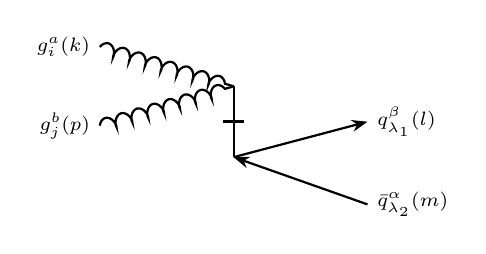
\begin{tikzpicture}
\draw[gl] (0,2.0) -- (1.7,1.5); \node[left] at (0,2.0) {\scriptsize$\gl{a}{i}{k}$};
\draw[gl] (0,1.0) -- (1.7,1.5); \node[left] at (0,1.0) {\scriptsize$\gl{b}{j}{p}$};
\draw[ins] (1.7,1.5) -- (1.7,0.6); \ibar{1.7}{1.05}
\draw[qk] (1.7,0.6) -- (3.4,1.05); \node[right] at (3.4,1.05) {\scriptsize$\qk{\beta}{\lambda_{1}}{l}$};
\draw[qk] (3.4,0.0) -- (1.7,0.6); \node[right] at (3.4,0.0) {\scriptsize$\aqk{\alpha}{\lambda_{2}}{m}$};
\end{tikzpicture}
\end{center}
Charges: pair creation $t^{c}_{\beta\alpha}\delta_{\lambda_{1}\lambda_{2}}$ and two-gluon
annihilation, the conjugate of the creation entry, $-if^{cab}(p^{+}-k^{+})\delta_{ij}/
2\sqrt{k^{+}p^{+}}$; $P^{+}=k^{+}+p^{+}$:
\begin{res}
\begin{equation}
\psi_{\rm C2}=-\,\frac{i\,g^{2}\,f^{cab}\,t^{c}_{\beta\alpha}\,
\delta_{\lambda_{1}\lambda_{2}}\,\delta_{ij}\,(p^{+}-k^{+})\;\dthree(k+p-l-m)}
{2\,(2\pi)^{3}\sqrt{k^{+}p^{+}}\;(k^{+}+p^{+})^{2}\;
\big(\eps_{k}+\eps_{p}-\eps_{l}-\eps_{m}\big)} .
\label{eq:C2}
\end{equation}
\end{res}
\noindent
The remaining possibility, $\vac\to\ket{q\bar q\,gg}$, is forbidden: with no valence charge to
absorb momentum, four outgoing quanta with $p^{+}>0$ cannot conserve $p^{+}$.

%=====================================================================
\section{Group D: instantaneous quark exchange ($H_{ggq\bar q}$)}
%=====================================================================

Here the exchanged line is a fermion. The rule is the standard light-cone one: the instantaneous
fermion carries $\gamma^{+}/2P^{+}_{\rm inst}$, which in the two-component form becomes
$\sigma^{i}\,(2P^{+}_{\rm inst})^{-1}\,\sigma^{j}$ between the two gluon attachments, with
$P^{+}_{\rm inst}$ the $+$ momentum flowing along the barred line.

\subsection*{D1. \ $\ket{gg}\to\ket{q\bar q}$ \quad (feeds $\B_{1}$)}
\begin{center}
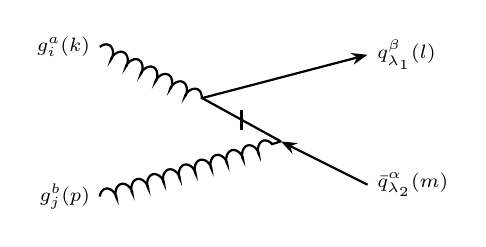
\begin{tikzpicture}
\draw[gl] (0,2.0) -- (1.3,1.35); \node[left] at (0,2.0) {\scriptsize$\gl{a}{i}{k}$};
\draw[gl] (0,0.1) -- (2.3,0.8); \node[left] at (0,0.1) {\scriptsize$\gl{b}{j}{p}$};
\draw[qk] (1.3,1.35) -- (3.4,1.9); \node[right] at (3.4,1.9) {\scriptsize$\qk{\beta}{\lambda_{1}}{l}$};
\draw[ins] (1.3,1.35) -- (2.3,0.8); \ibarh{1.8}{1.075}
\draw[qk] (3.4,0.25) -- (2.3,0.8); \node[right] at (3.4,0.25) {\scriptsize$\aqk{\alpha}{\lambda_{2}}{m}$};
\end{tikzpicture}
\end{center}
The two orderings of the gluon attachments give $P^{+}_{\rm inst}=l^{+}-k^{+}$ and
$l^{+}-p^{+}$:
\begin{res}
\begin{equation}
\psi_{\rm D1}=\frac{g^{2}\,\dthree(k+p-l-m)}
{16\pi^{3}\sqrt{k^{+}p^{+}}\;\big(\eps_{k}+\eps_{p}-\eps_{l}-\eps_{m}\big)}\;
\chi^{\dg}_{\lambda_{1}}\!\left[
\frac{(t^{a}t^{b})_{\beta\alpha}\,\sigma^{i}\sigma^{j}}{l^{+}-k^{+}}
+\frac{(t^{b}t^{a})_{\beta\alpha}\,\sigma^{j}\sigma^{i}}{l^{+}-p^{+}}\right]\chi_{\lambda_{2}} .
\label{eq:D1}
\end{equation}
\end{res}

\subsection*{D2. \ $\ket{g}\to\ket{q\bar q\,g}$ \quad (feeds $\B_{3}$)}
\begin{center}
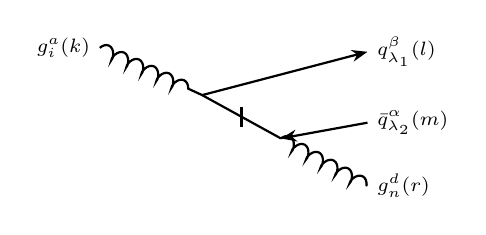
\begin{tikzpicture}
\draw[gl] (0,1.9) -- (1.3,1.3); \node[left] at (0,1.9) {\scriptsize$\gl{a}{i}{k}$};
\draw[gl] (2.3,0.75) -- (3.4,0.15); \node[right] at (3.4,0.15) {\scriptsize$\gl{d}{n}{r}$};
\draw[qk] (1.3,1.3) -- (3.4,1.85); \node[right] at (3.4,1.85) {\scriptsize$\qk{\beta}{\lambda_{1}}{l}$};
\draw[ins] (1.3,1.3) -- (2.3,0.75); \ibarh{1.8}{1.025}
\draw[qk] (3.4,0.95) -- (2.3,0.75); \node[right] at (3.4,0.95) {\scriptsize$\aqk{\alpha}{\lambda_{2}}{m}$};
\end{tikzpicture}
\end{center}
Now one gluon is incoming and one outgoing, so $P^{+}_{\rm inst}=l^{+}+r^{+}$ when the outgoing
gluon attaches on the quark side and $-(m^{+}+r^{+})$ when it attaches on the antiquark side:
\begin{res}
\begin{equation}
\psi_{\rm D2}=\frac{g^{2}\,\dthree(k-l-m-r)}
{16\pi^{3}\sqrt{k^{+}r^{+}}\;\big(\eps_{k}-\eps_{l}-\eps_{m}-\eps_{r}\big)}\;
\chi^{\dg}_{\lambda_{1}}\!\left[
\frac{(t^{d}t^{a})_{\beta\alpha}\,\sigma^{n}\sigma^{i}}{l^{+}+r^{+}}
-\frac{(t^{a}t^{d})_{\beta\alpha}\,\sigma^{i}\sigma^{n}}{m^{+}+r^{+}}\right]\chi_{\lambda_{2}} .
\label{eq:D2}
\end{equation}
\end{res}

\subsection*{D3. \ $\ket{q\,g}\to\ket{q\,g}$}
\begin{center}
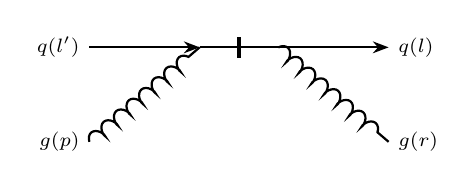
\begin{tikzpicture}
\draw[qk] (0,1.6) -- (1.4,1.6); \node[left] at (0,1.6) {\scriptsize$q(l')$};
\draw[gl] (0,0.4) -- (1.4,1.6); \node[left] at (0,0.4) {\scriptsize$g(p)$};
\draw[ins] (1.4,1.6) -- (2.4,1.6); \ibarh{1.9}{1.6}
\draw[qk] (2.4,1.6) -- (3.8,1.6); \node[right] at (3.8,1.6) {\scriptsize$q(l)$};
\draw[gl] (2.4,1.6) -- (3.8,0.4); \node[right] at (3.8,0.4) {\scriptsize$g(r)$};
\end{tikzpicture}
\end{center}
Instantaneous quark exchange in the $q g$ channel. The structure is $a^{\dg}a\,b^{\dg}b$, which is
\emph{not in the ansatz}: it contributes only when $\Omega$ acts on states containing both a soft
gluon and a soft quark. Recorded for completeness.

%=====================================================================
\section{Summary}
%=====================================================================

\begin{center}
\renewcommand{\arraystretch}{1.3}
\begin{tabular}{clllc}
\hline
& transition & origin & feeds & in the draft?\\
\hline
A1 & $\vac\to q\bar q$ & $\rho\!\cdot\!\Jc_{q}$ & $\A_{1}$ & yes, Eq.~(22)\\
A2 & $q\bar q\to q\bar q$ (quark leg) & $\rho\!\cdot\!\Jc_{q}$ & $b^{\dg}b$, $\D_{3}$ & no\\
A3 & $q\bar q\to q\bar q$ (antiquark leg) & $\rho\!\cdot\!\Jc_{q}$ & $d^{\dg}d$, $\D_{3}$ & no\\
A4 & $g\to g\,q\bar q$ (spectator) & $\rho\!\cdot\!\Jc_{q}$ & disconnected ($\A_{1}$) & implicitly\\
B1 & $q\bar q\to q\bar q$ & $\Jc_{q}\!\cdot\!\Jc_{q}$ & $\D_{3}$ & no\\
B2 & $\vac\to q\bar q\,q\bar q$ & $\Jc_{q}\!\cdot\!\Jc_{q}$ & beyond the ansatz & no\\
C1 & $g\to q\bar q\,g$ & $\Jc_{q}\!\cdot\!\Jc_{g}$ & $\B_{3}$ & \textbf{no --- new}\\
C2 & $gg\to q\bar q$ & $\Jc_{q}\!\cdot\!\Jc_{g}$ & $\B_{1}$ & \textbf{no --- new}\\
D1 & $gg\to q\bar q$ & $H_{ggq\bar q}$ & $\B_{1}$ & no\\
D2 & $g\to q\bar q\,g$ & $H_{ggq\bar q}$ & $\B_{3}$ & no\\
D3 & $q\,g\to q\,g$ & $H_{ggq\bar q}$ & beyond the ansatz & no\\
\hline
\end{tabular}
\end{center}

\noindent
Of the eleven instantaneous topologies, exactly one --- A1 --- appears in the current draft.
Four (A4, B1, D1, D2) were restored in the corrected manuscript. Two (C1, C2) are identified here
for the first time and need to be added to $\B_{3}$ and $\B_{1}$. Three (A2, A3, D3) populate
operator structures that the ansatz does not contain, and B2 likewise; they are inert for the
matching sectors used so far, but must be restored before $\Omega$ is applied to states
containing both soft gluons and soft quarks.

\medskip\noindent
Two structural remarks. First, writing the instantaneous gluon exchange as the single
current--current operator \eqref{eq:HinstA} rather than as a list of separate Hamiltonians is what
makes the enumeration exhaustive: one simply expands $\Jc=\rho+\Jc_{g}+\Jc_{q}$ and reads off the
cross terms. The two missing topologies C1 and C2 are exactly the ones that a
list-of-Hamiltonians organization loses. Second, every graph in Groups A--C collapses onto the
single rule \eqref{eq:rule}, so only the charges and $P^{+}$ need to be identified in each case.

\end{document}
